\documentclass{article}

\usepackage{graphicx}
\usepackage[margin=1in]{geometry}
\usepackage{subcaption}
\usepackage[justification=centering]{caption}
\usepackage{hyperref}
\usepackage{siunitx}
\usepackage{tikz} % To generate the plot from csv
\usepackage{pgfplots}

\pgfplotsset{compat=newest} % Allows to place the legend below plot
\usepgfplotslibrary{units} % Allows to enter the units nicely

\title{Lattice Boltzmann simulation of evaporating droplet}
\date{CH13B006}
\author{Aqel Ahammad K P}
\newpage


\begin{document}
\begin{titlepage}
			\centering
			
\includegraphics[width=0.15\textwidth]{images/others/iitm_logo}\par\vspace{1cm}
			{\scshape\LARGE IIT Madras \par}
			\vspace{1cm}
			{\scshape\Large Final year BTech Project\par}
			\vspace{1.5cm}
			{\huge\bfseries Lattice Boltzmann simulation of evaporating droplet\par}
			\vspace{2cm}
			{\Large\itshape Aqel Ahammad K P\par}
			{\Large\itshape CH13B006\par}
			\vfill
			Guided by\par
			Prof. Sumesh Thampi
			
			\vfill
			
			% Bottom of the page
			{\large \today\par}
		\end{titlepage}
\tableofcontents
\pagenumbering{roman}
\newpage
\pagenumbering{arabic}

\section{Abstract}
Evaporation and condensation is modeled in this study using two methods - Lattice Boltzmann method and Method of lines. These two methods were evaluated based on space and time complexity, average time for one iteration and time for convergence. Evaporation of planar droplet was simulated and reproduced results mentioned in the literature. The boundary condition for evaporation was reversed for initiating condensation and was able to bring opposite effect. Evaporation and condensation of a sessile droplet was studied on ideal and hysteritic surfaces. The results showed same pattern that is recorded experimentally. Pinning of contact line during evaporation was achieved on a hysteretic surface by defining a smaller receding angle. 

\section{Governing equations}
Continuity equation,
\begin{equation}
	\frac{\partial \rho}{\partial t} + \nabla.(\rho \vec{v}) = 0
\label{eq:continuity}
\end{equation}
Navier-Stokes equation,
\begin{equation}
	%{\partial{\vec{v}}\over{\partial t}} + ({\vec{v}} \cdot \nabla) {\vec{v}} = - {1\over\rho} \nabla p + \gamma\nabla^2{\vec{v}} + {1\over\rho}{\vec{F} }
	\rho [\vec{v} + (\vec{v}.\nabla)\vec{v}] = \eta \nabla^2\vec{v}-\phi\nabla\mu - \nabla P
	\label{eq:NS}
\end{equation}
Cahn-Hilliard convection-diffusion equation,
\begin{equation}
	\frac{\partial \phi}{\partial t} = \nabla.(\phi \vec{v}) + \nabla.(M\nabla\phi)
 \label{eq:CH}
\end{equation}
where $\phi$ is the phase field and M is \textit{mobility parameter} which plays the role of diffusivity.

\section{Lattice-Boltzmann method}
Instead of solving equations (\ref{eq:continuity})-(\ref{eq:CH}), the discrete Boltzmann equation is solved to simulate the flow of a Newtonian fluid.
\begin{equation}
	f_{i}(\textbf{r}+\textbf{c}_{i}\Delta t, t+\Delta t) - f_{i}(\textbf{r},t) = -\frac{\Delta t}{\tau}(f_{i}-f_{i}^{eq})
	\label{eq:f}
\end{equation}

\begin{equation}
g_{i}(\textbf{r}+\textbf{c}_{i}\Delta t, t+\Delta t) - g_{i}(\textbf{r},t) = -\frac{\Delta t}{\tau_{g}}(g_{i}-g_{i}^{eq})
\label{eq:g}
\end{equation}

Hydrodynamic variables are related to above velocity distribution functions by,
\begin{equation}
	\rho \equiv \sum_{i} f_{i}, \quad \rho v_{\alpha} \equiv \sum_{i} c_{i\alpha} f_{i}, \quad \phi \equiv \sum_{i} g_{i}
	\label{eq:fg}
\end{equation}

Also, 
\begin{equation}
 \sum_{i} f_{i}^{eq} \equiv \rho, \quad \  \sum_{i} c_{i\alpha} f_{i}^{eq} \equiv rho v_{\alpha}, \sum_{i} g_{i}^{eq} \equiv \quad \phi 
\label{eq:fg}
\end{equation}
Expressions for equilibrium distribution functions are reported in \cite{paper:intertial_effects}.

\section{LB Method and Method of Lines}
Equation (\ref{eq:CH}) can be solved using method of lines. In this section, we compare various aspects of algorithms of LB method(LBM) and method of lines(MOL)
\subsection*{Time complexity}
Average time required for one iteration in both the algorithms was noted and plotted in Figure \ref*{fig:lbm_vs_mol_time}. It was noted that time for one iteration of MOL is almost equal to LB method with D2Q9 lattice. Time varies linearly with number of points for both the algorithms. Hence both shows time complexity of $\mathcal{O}(n)$
\begin{figure}[h!]
	%\begin{center}
	\begin{subfigure}{7cm}
		\begin{tikzpicture}
		\begin{axis}[
		width=7cm, % Scale the plot to \linewidth
		grid=major, % Display a grid
		grid style={dashed,gray!30}, % Set the style
		xlabel=Number of points, % Set the labels
		ylabel=Average time for one iteration,
		%x unit=\si{\volt}, % Set the respective units
		%y unit=\si{\ampere},
		%legend style={at={( 1.01,1)}, anchor=north west}, % Put the legend below the plot
		x tick label style={rotate=90,anchor=east} % Display labels sideways
		]
		\addplot 
		[only marks]
		table[x=points,y=lbm,col sep=comma] {data/lbm_vs_mol_time.csv}; 
		%\addlegendentry{LB Method}
		\addplot
		[color=red] 
		[only marks]
		table[x=points,y=mol,col sep=comma] {data/lbm_vs_mol_time.csv}; 
		%\addlegendentry{Method of Lines}
		
		\end{axis}
		
		\end{tikzpicture}
		\caption{Average time for one iteration vary linearly for both the methods}
		\label{fig:lbm_vs_mol_time}
	\end{subfigure}
	\begin{subfigure}{7cm}
		\begin{tikzpicture}
		\begin{axis}[
		width=7cm, % Scale the plot to \linewidth
		grid=major, % Display a grid
		grid style={dashed,gray!30}, % Set the style
		xlabel=Time, % Set the labels
		ylabel=RMS Error,
		%x unit=\si{\volt}, % Set the respective units
		%y unit=\si{\ampere},
		legend style={at={( 1.05,0.6)}, anchor=north west}, % Put the legend below the plot
		x tick label style={rotate=90,anchor=east} % Display labels sideways
		]
		\addplot 
		[color=black]
		table[x=time,y=lbm,col sep=comma] {data/time_convergence.csv}; 
		\addlegendentry{LB Method}
		\addplot
		[color=red] 
		table[x=time,y=mol,col sep=comma] {data/time_convergence.csv}; 
		\addlegendentry{Method of Lines}
		
		\end{axis}
		
		\end{tikzpicture}
		\caption{Both the algorithms show same time for convergence}
		\label{fig:lbm_vs_mol_convergence}
	\end{subfigure}
	\caption{Time complexity and convergence analysis for LB method and method of lines}
	\label{fig:lbm_vs_mol}
	%\end{center}
	
\end{figure}
\subsection*{Space complexity}
Both the algorithms have same space complexity  $\mathcal{O}(n)$
\subsection*{Time for convergence}
It was noted that both the methods gives almost same result and error at a particular time and takes almost same time to converge to a solution. 




\section{Spinodal decomposition}

Spinodal decomposition is a mechanism for the rapid unmixing of a mixture of liquids or solids from one thermodynamic phase, to form two coexisting phases. Refer Figure \ref*{fig:spinod} for the spinodal decomposition simulation where we started with each point having a random $\phi$ value where $ -1 \leq \phi \leq 1.  $
\begin{figure}[h!]
	\centering
	\begin{subfigure}[h!]{4cm}            
		\frame{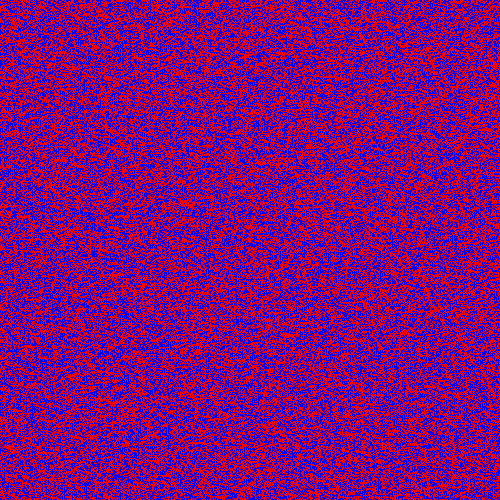
\includegraphics[width=4cm]{images/spinodal/0.png}}
		\caption{t = 0}
		\label{Fig:Data1}
	\end{subfigure}
	\begin{subfigure}[h!]{4cm}
		\centering
		\frame{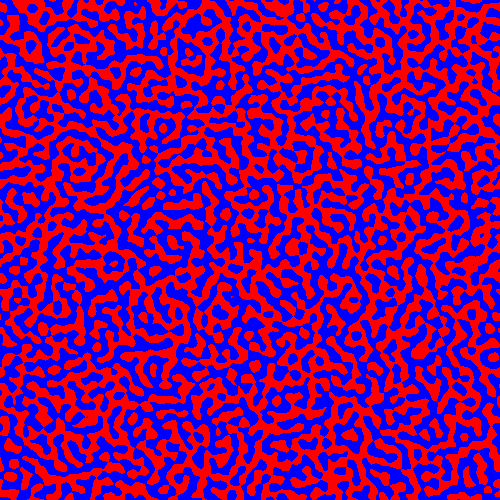
\includegraphics[width=4cm]{images/spinodal/1000.png}}
		\caption{t = 1000}
		\label{Fig:Data2}
	\end{subfigure}
	\begin{subfigure}[h!]{4cm}            
		\frame{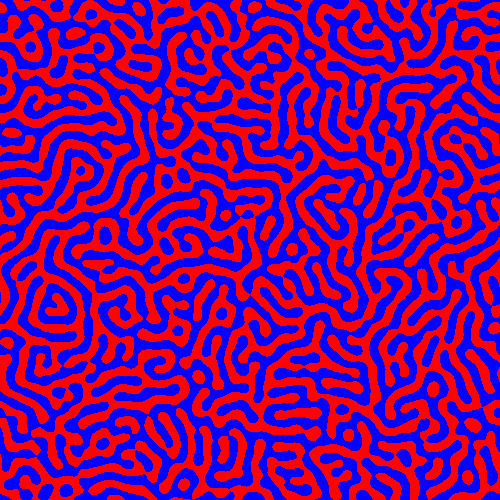
\includegraphics[width=4cm]{images/spinodal/10000.png}}
		\caption{t = 10000}
		\label{Fig:Data3}
	\end{subfigure}
	\begin{subfigure}[h!]{4cm}
		\centering
		\frame{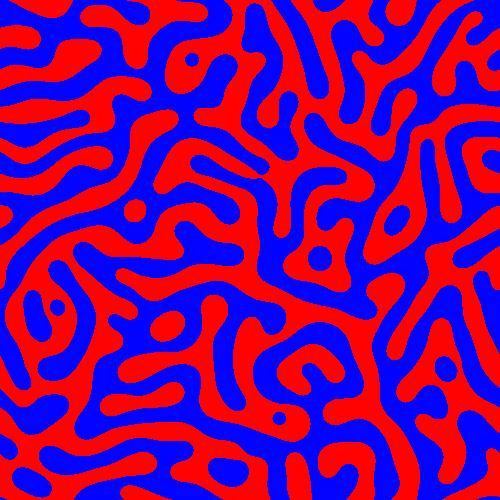
\includegraphics[width=4cm]{images/spinodal/100000.png}}
		\caption{t = 100000}
		\label{Fig:Data4}
	\end{subfigure}
	\caption{Spinodal decomposition simulation in a domain of 500 * 500 using Lattice Boltzmann method. It can be seen that phases unmix to form separate clusters.}\label{fig:spinod}
\end{figure}
\begin{flushright}
	\href{https://www.youtube.com/watch?v=B9JiYVE437Y}{[Click here to see the video of the simulation.]}
\end{flushright}
   
\section{Surface tension}
Surface tension is the elastic tendency of a fluid surface which makes it acquire the least surface area possible. For any volume, sphere gives the least surface area. In the following simulation, a cubic volume of liquid is taken at t = 0. As expected, the droplets changes itself to a spherical droplet. (Refer Figure \ref{fig:surface_tension})

\begin{figure}[h!]
	\centering
	\begin{subfigure}[h!]{5cm}            
		\frame{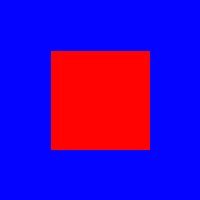
\includegraphics[width=5cm]{images/surface_tension/0.png}}
		\caption{At t = 0}
		\label{Fig:surface_initial}
	\end{subfigure}
	\begin{subfigure}[h!]{5cm}
		\centering
		\frame{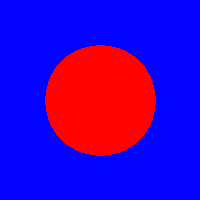
\includegraphics[width=5cm]{images/surface_tension/880000.png}}
		\caption{At equilibrium }
		\label{Fig:surface_final}
	\end{subfigure}
	\caption{Evolution of a square surface to a circular surface.}\label{fig:surface_tension}
\end{figure}

\section{Variation of phase field close to interfase}
Close to interface, the phase field varies as a hyperbolic tangent with the normal coordinates to the interface, r. Simulation data was perfectly matching with the numerical solution given by \cite{arXiv:1104.0078}. (Refer Fig \ref*{fig:tanh}) \newline
\begin{equation}
	\phi(r) = \phi_{eq}tan h(\frac{r}{\epsilon})
\end{equation}
where $\phi_{eq} = \sqrt{-a/b}$ and $\epsilon \equiv \sqrt{-2k/a}$ is the interface thickness
\begin{figure}[h!]
	\begin{center}
		\begin{tikzpicture}
		\begin{axis}[
		width=7cm, % Scale the plot to \linewidth
		grid=major, % Display a grid
		grid style={dashed,gray!30}, % Set the style
		xlabel=$x$, % Set the labels
		ylabel=$\phi(x)/\phi_{eq}$,
		%x unit=\si{\volt}, % Set the respective units
		%y unit=\si{\ampere},
		legend style={at={( 1.01,1)}, anchor=north west}, % Put the legend below the plot
		x tick label style={rotate=90,anchor=east} % Display labels sideways
		]
		\addplot 
		% add a plot from table; you select the columns by using the actual name in
		% the .csv file (on top)
		table[x=X,y=Y,col sep=comma] {data/tanh.csv}; 
		\addlegendentry{Simulation data}
		\addplot [
		domain=0:150, 
		samples=100, 
		color=red,
		]
		%{abs(tanh(deg(x)))};
		{tanh((75-x)/2.2615822112761355)};
		\addlegendentry{Numerical Solution}
		\end{axis}
		
		\end{tikzpicture}
		\caption{Phase field profile along normal to interface of two already separated phases }
		\label{fig:tanh}
	\end{center}

\end{figure}

\section{Solid wall}
Bounce-back rules \cite{paper:bounce_back} are imposed along the boundary for impenetrability and no-slip boundary conditions. Also,
\begin{equation}
	\vec{n}.\nabla\mu = 0
\end{equation}
 For an equilibrium contact angle on an ideal solid wall, geometrical formulation is used for implementing wetting condition \cite{paper:contact_angle,PhysRevE.75.046708}.
 \begin{equation}
 \phi_{i,j,1} = \phi_{i,j,3} + tanh(\frac{\pi}{2}-\theta) \xi
 \end{equation}
 where 
 \begin{equation}
 	\xi = \sqrt{(\phi_{i+1,j,2}-\phi_{i-1,j,2})^{2}+(\phi_{i,j+1,2}-\phi_{i,j-1,2})^{2}}
 \label{eqn_wetting_bc}
 \end{equation}
 \begin{figure}[h!]
 	\centering
 	\begin{subfigure}{3.7cm}
 		\frame{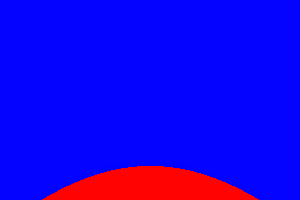
\includegraphics[height=3cm,trim=1cm 0 1cm 0, clip]{images/solid_wall/30.png}}
 		\caption{30$ ^{0} $}
 	\end{subfigure}
 	\begin{subfigure}{3cm}            
 		\frame{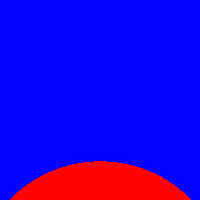
\includegraphics[width=3cm]{images/solid_wall/45.png}}
 		\caption{45$ ^{0} $}
 		\label{Fig:Datsa3}
 	\end{subfigure}
 	
 	\begin{subfigure}{3cm}
 		\frame{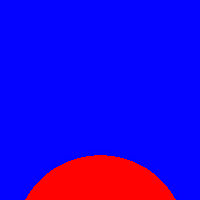
\includegraphics[width=3cm]{images/solid_wall/60.png}}
 		\caption{60$ ^{0} $}
 	\end{subfigure}
 	\begin{subfigure}[h!]{3cm}            
 		\frame{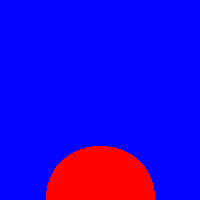
\includegraphics[width=3cm]{images/solid_wall/90.png}}
 		\caption{90$ ^{0} $}
 		\label{Fig:Datsa1}
 	\end{subfigure}
 	\begin{subfigure}[h!]{3cm}            
 		\frame{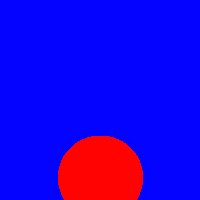
\includegraphics[width=3cm]{images/solid_wall/120.png}}
 		\caption{$ 120^{0} $}
 		\label{Fig:Datsase3}
 	\end{subfigure}
 	\begin{subfigure}[h!]{3cm}
 		\frame{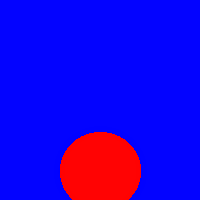
\includegraphics[width=3cm]{images/solid_wall/135.png}}
 		\caption{$ 135^{0} $}
 	\end{subfigure}
 	\begin{subfigure}[h!]{3cm}
	 	\frame{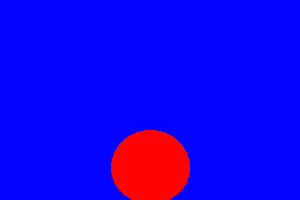
\includegraphics[height=3cm,trim=2cm 0 2cm 0, clip]{images/solid_wall/150.png}}
	 	\caption{150$ ^{0} $}
	\end{subfigure}
 	\caption{Droplets on solid wall with different contact angles }
 	\label{fig:spinods}
 \end{figure}

\section{Evaporation of a planar droplet}

To drive evaporation of the film we impose the boundary condition $\phi(z=z_{H},t)=\phi_{H}$, where $\phi_{H} < -\phi_{eq}$. This induces a gradient in the chemical potential field $\mu$. In response to this imbalance, the system reduces $\phi$, which corresponds to the evaporation of the film\cite{paper:evaporation}.
Phase field imbalance, $\Delta\phi_{H} \equiv -\phi_{eq} - \phi_{H}$
\newline
We performed simulations in a box consisting of  1 x 1 x 150 lattice sites. Periodic boundary conditions were set in the x and
y directions. A wall was located at $ z_{w} = 1 $, while the concentration
was fixed to a value $ \phi_{H}$ at $z_{H} = N_{z} $ to drive the system out of equilibrium. The initial height of the film was set to $z_{0} = 100$. 

\begin{figure}[h!]
	\begin{center}
		\begin{subfigure}{6cm}
			\begin{tikzpicture}
			\begin{axis}[
			width=6cm, % Scale the plot to \linewidth
			grid=major, % Display a grid
			grid style={dashed,white!30}, % Set the style
			xlabel=$z$, % Set the labels
			ylabel=$\phi(x)/\phi_{eq}$,
			%x unit=\si{\volt}, % Set the respective units
			%y unit=\si{\ampere},
			%legend style={at={( 1.01,1)}, anchor=north west}, % Put the legend below the plot
			no markers,
			every axis plot/.append style={ultra thick},
			x tick label style={rotate=90,anchor=east} % Display labels sideways
			]
			\addplot 
			table[x=y,y=0.3,col sep=comma] {data/evaporation_different_phih.csv}; 
			\addlegendentry{0.3}
			\addplot 
			table[x=y,y=0.4,col sep=comma] {data/evaporation_different_phih.csv}; 
			\addlegendentry{0.4}
			\addplot 
			table[x=y,y=0.2,col sep=comma] {data/evaporation_different_phih.csv}; 
			\addlegendentry{0.2}
			\addplot 
			[color=cyan]
			table[x=y,y=0.1,col sep=comma] {data/evaporation_different_phih.csv}; 
			\addlegendentry{0.1}
			
			\end{axis}
			\end{tikzpicture}
			\caption{After 5 x $10^{6}$ simulation steps with different $\phi_{H}$}
			\label{fig:evaporation_tanh}
		\end{subfigure}
		\quad 
		\begin{subfigure}{6cm}
			\begin{tikzpicture}
			\begin{axis}[
			width=6cm, % Scale the plot to \linewidth
			grid=major, % Display a grid
			grid style={dashed,white!30}, % Set the style
			xlabel=$z$, % Set the labels
			ylabel=$\phi(x)/\phi_{eq}$,
			%x unit=\si{\volt}, % Set the respective units
			%y unit=\si{\ampere},
			legend style={at={( 1.01,1)}, anchor=north west}, % Put the legend below the plot
			no markers,
			every axis plot/.append style={ultra thick},
			x tick label style={rotate=90,anchor=east} % Display labels sideways
			]
			\addplot 
			table[x=y,y=1,col sep=comma] {data/evaporation_time.csv}; 
			\addlegendentry{$10^{5}$}
			\addplot 
			table[x=y,y=3,col sep=comma] {data/evaporation_time.csv}; 
			\addlegendentry{3 x $10^{5}$}
			\addplot 
			table[x=y,y=5,col sep=comma] {data/evaporation_time.csv}; 
			\addlegendentry{5 x $10^{5}$}
			\addplot 
			table[x=y,y=7,col sep=comma] {data/evaporation_time.csv}; 
			\addlegendentry{7 x $10^{5}$}
			
			\end{axis}
			\end{tikzpicture}
		\caption{Phase field profile at different time steps}
		\label{fig:evaporation_time}
		
		\end{subfigure}
		\caption{Phase field profile for the planar film evaporation. }
		\label{fig:evaporation_different_phih}
	\end{center}
	
\end{figure}

\section{Condensation of planar droplet}
Similar to evaporation, condensation can be simulated by imposing boundary condition $\phi(z=z_{H},t)=\phi_{H}$, where $\phi_{H} > -\phi_{eq}$.
\begin{figure}[h!]
	\begin{center}
		\begin{tikzpicture}
		\begin{axis}[
		width=7cm, % Scale the plot to \linewidth
		grid=major, % Display a grid
		grid style={dashed,gray!30}, % Set the style
		xlabel=$x$, % Set the labels
		ylabel=$\phi(x)/\phi_{eq}$,
		%x unit=\si{\volt}, % Set the respective units
		%y unit=\si{\ampere},
		legend style={at={( 1.01,1)}, anchor=north west}, % Put the legend below the plot
		x tick label style={rotate=90,anchor=east} % Display labels sideways
		]
		\addplot 
		table[x=t,y=before_evaporation,col sep=comma] {data/evaporation_condensation_1D.csv}; 
		\addlegendentry{Before evaporation}
		\addplot 
		table[x=t,y=after_evaporation,col sep=comma] {data/evaporation_condensation_1D.csv}; 
		\addlegendentry{After evaporation}
		\addplot 
		table[x=t,y=before_cond,col sep=comma] {data/evaporation_condensation_1D.csv}; 
		\addlegendentry{Before condensation}
		\addplot 
		table[x=t,y=after_cond,col sep=comma] {data/evaporation_condensation_1D.csv}; 
		\addlegendentry{After condensation}
		\end{axis}
		
		\end{tikzpicture}
		\caption{Phase field profile along normal to interface of evaporating and condensing planar droplet.  }
		\label{fig:evap_cond_1D}
	\end{center}
	
\end{figure}
In Figure \ref*{fig:evap_cond_1D}, a planar droplet of height 100 is evaporated with $\phi_{H} = -1.1$. After $5 x 10^{6}$ timesteps, boundary condition at z = 150 is changed to $\phi_{H} = -0.245$ ( at which $\mu$ is equal and opposite to that of $\mu(\phi=-1.1)$ ) to initiate evaporation. It is observed that after condensing for same duration as that of evaporation, at $t = 10 x 10^{6}$ the system returns to the initial condition. 

\section{Evaporation and condensation of a sessile droplet on a solid surface}

\subsection{Ideal surface}
\begin{figure}[h!]
	\begin{center}
		\begin{tikzpicture}
		\begin{axis}[
		ticks=none,
		width=6cm, % Scale the plot to \linewidth
		%grid=major, % Display a grid
		%grid style={dashed,gray!30}, % Set the style
		%xlabel=$x$, % Set the labels
		%ylabel=$\phi(x)/\phi_{eq}$,
		%x unit=\si{\volt}, % Set the respective units
		%y unit=\si{\ampere},
		legend style={at={( 1.01,1)}, anchor=north west}, % Put the legend below the plot
		no markers,
		every axis plot/.append style={ultra thick},
		x tick label style={rotate=90,anchor=east}, % Display labels sideways
		xticklabels={,,},
		yticklabels={,,}		
		]
		\addplot 
		[color=black]
		table[x=0x,y=0y,col sep=comma] {data/evaporation_ideal_outline.csv}; 
		
	
		
		\addplot 
		[color=black]
		table[x=2x,y=2y,col sep=comma] {data/evaporation_ideal_outline.csv}; 
		
		\addplot 
		[color=black]
		table[x=3x,y=3y,col sep=comma] {data/evaporation_ideal_outline.csv}; 
		\end{axis}		
		\end{tikzpicture}
		\caption{Shape profile of an evaporating droplet on an ideal surface. }
		\label{fig:evpn_outline}
	\end{center}
	
\end{figure}

An ideal solid surface is flat, rigid, perfectly smooth, and chemically homogeneous, and has zero contact angle hysteresis. On such a surface, only one thermodynamically stable contact angle exists. Hence we expect a constant contact angle and varying contact diameter during evaporation and condensation. 
\begin{figure}[h!]
	\begin{center}
		
		\begin{subfigure}{6cm}
			\begin{tikzpicture}
			\begin{axis}[
			width=6cm, % Scale the plot to \linewidth
			grid=major, % Display a grid
			grid style={dashed,white!30}, % Set the style
			xlabel=$t$, % Set the labels
			%ylabel=$t$,
			%x unit=\si{\volt}, % Set the respective units
			%y unit=\si{\ampere},
			%legend style={at={( 1.01,1)}, anchor=north west}, % Put the legend below the plot
			no markers,
			every axis plot/.append style={ultra thick},
			x tick label style={rotate=90,anchor=east} % Display labels sideways
			]
			\addplot 
			table[x=t,y=diameter, col sep=comma] {data/condensation_90.csv}; 
			\addlegendentry{Contact diameter}
			\addplot 
			table[x=t,y=slope,col sep=comma] {data/condensation_90.csv}; 
			\addlegendentry{Contact angle}
			\addplot 
			table[x=t,y=height,col sep=comma] {data/condensation_90.csv}; 
			\addlegendentry{Drop height}
			\legend{}; % empty the legend so as not to print it
			\end{axis}
			\end{tikzpicture}
			\caption{Condensation}
			\label{fig:cond_90}
			
		\end{subfigure}
		
		\quad 
		\begin{subfigure}{6cm}
			\begin{tikzpicture}
			\begin{axis}[
			width=6cm, % Scale the plot to \linewidth
			grid=major, % Display a grid
			grid style={dashed,white!30}, % Set the style
			xlabel=$t$, % Set the labels
			%ylabel=$t$,
			%x unit=\si{\volt}, % Set the respective units
			%y unit=\si{\ampere},
			legend style={at={( 1.01,1)}, anchor=north west}, % Put the legend below the plot
			no markers,
			every axis plot/.append style={ultra thick},
			x tick label style={rotate=90,anchor=east} % Display labels sideways
			]
			\addplot 
			table[x=t,y=diameter, col sep=comma] {data/evaporation_90.csv}; 
			\addlegendentry{Contact diameter}
			\addplot 
			table[x=t,y=slope,col sep=comma] {data/evaporation_90.csv}; 
			\addlegendentry{Contact angle}
			\addplot 
			table[x=t,y=height,col sep=comma] {data/evaporation_90.csv}; 
			\addlegendentry{Drop height}
			\end{axis}
			\end{tikzpicture}
			\caption{Evaporation}
			\label{fig:evpn_90}
			
		\end{subfigure}
		
		\caption{Contact diameter, angle and drop height of a droplet on an ideal surface with equilibrium contact angle $90^{0}$ during evaporation/condensation. }
		\label{fig:evpn_ideal}
	\end{center}
	
\end{figure}



\subsection{Hysteretic surface}
\begin{figure}[h!]
	\begin{center}
		\begin{tikzpicture}
		\begin{axis}[
		ticks=none,
		width=6cm, % Scale the plot to \linewidth
		%grid=major, % Display a grid
		%grid style={dashed,gray!30}, % Set the style
		%xlabel=$x$, % Set the labels
		%ylabel=$\phi(x)/\phi_{eq}$,
		%x unit=\si{\volt}, % Set the respective units
		%y unit=\si{\ampere},
		legend style={at={( 1.01,1)}, anchor=north west}, % Put the legend below the plot
		no markers,
		every axis plot/.append style={ultra thick},
		x tick label style={rotate=90,anchor=east}, % Display labels sideways
		xticklabels={,,},
		yticklabels={,,}		
		]
		\addplot 
		[color=black]
		table[x=0x,y=0y,col sep=comma] {data/evaporation_hysteritic_outline.csv}; 
		
		
		
		\addplot 
		[color=black]
		table[x=2x,y=2y,col sep=comma] {data/evaporation_hysteritic_outline.csv}; 
		
		\addplot 
		[color=black]
		table[x=1x,y=1y,col sep=comma] {data/evaporation_hysteritic_outline.csv}; 
		\end{axis}		
		\end{tikzpicture}
		\caption{Shape profile of an evaporating droplet on a hysteretic surface. }
		\label{fig:evpn_hysteritic_outline}
	\end{center}
\end{figure}

In many natural systems, the solid walls are usually rough and chemically inhomogeneous. In these surfaces, contact angle hysteresis has to be taken into consideration. Due to hysteresis, the contact line remains pinned when the local contact angle $\theta$ is within a hysteresis window.
\begin{equation}
\theta_{R} \leq \theta \leq \theta_{A} 
\end{equation}
where $\theta_{R}$ and $\theta_{A}$ denote the receding angle and advancing angle respectively. 
\newline
When $\theta$ is greater than $\theta_{A}$, the contact line moves forward. When $\theta$ is less than $\theta_{R}$, the contact line moves backward. To realize this effect, at each time step of computation, we should first obtain the local apparent contact angle at the contact points. Then, comparisons of $\theta$ with $\theta_{R}$ and $\theta_{A}$ are required. If $\theta \leq \theta_{R}$, $\theta$ in Eq.\ref{eqn_wetting_bc} should be replaced by $\theta_{R}$; if $\theta \geq \theta_{A}$, $\theta$ should be replaced by $\theta_{A}$; else $\theta$ in Eq.\ref{eqn_wetting_bc} remains unchanged.
\par
A small difference in contact angle imposed using Eq.\ref{eqn_wetting_bc} and measured contact angle was observed in the simulation. This difference was causing error while implementing contact angle hysteresis, i.e, the contact angle $\theta$ was reaching $\theta_{R}$ at a very short time causing contact angle pinning to be visible for very small duration. Hence, difference between measured angle and imposed angle was plotted in Figure \ref{fig:angle_correction} and this data was used to correct the measured angle. 
\begin{figure}[h!]
	\begin{center}
		\begin{tikzpicture}
		\begin{axis}[
		width=7cm, % Scale the plot to \linewidth
		grid=major, % Display a grid
		grid style={dashed,gray!30}, % Set the style
		xlabel=Imposed angle, % Set the labels
		ylabel=Difference,
		x unit=\si{\deg}, % Set the respective units
		y unit=\si{\deg},
		legend style={at={( 1.01,1)}, anchor=north west}, % Put the legend below the plot
		no markers,
		every axis plot/.append style={ultra thick},
		x tick label style={rotate=90,anchor=east}, % Display labels sideways
		]
		\addplot 
		table[x=angle,y=difference,col sep=comma] {data/error_data.csv}; 
		
		\end{axis}		
		\end{tikzpicture}
		\caption{Difference between imposed contact angle and measured contact angle}
		\label{fig:angle_correction}
	\end{center}
\end{figure}

\par
Picknett and Bexon\cite{PICKNETT1977336} followed the mass and profile evolution of organic liquid drops. They observed three
distinct evaporation modes: mode 1, during which the
solid and iquid interface area remains constant (when hysteresis
exists); mode 2, for which the contact angle remains
constant (ideal system with no hysteresis at equilibrium);
mode 3, which is a mixed mode. They also observed that evaporation follows the first mode until $\theta = \theta_{R}$, and then, the second mode is initiated.\cite{doi:10.1021/la00007a076}


\par
In Figure \ref*{fig:evpn_cah} a droplet with initial contact angle $90^{0}$ is evaporating on a surface with $\theta_{R} = 42^{0}$ and $\theta_{A} = 140^{0}$. It followes mode 1 in the initial stage where contact diameter stays constant whereas contact angle decreases. After contact angle reaches $\theta = \theta_{R}$, mode 2 is observed in which contact angle stays at $\theta_{R}$ and the contact diameter reduces. 
\begin{figure}[h!]
	\begin{center}
		\begin{tikzpicture}
		\begin{axis}[
		width=7cm, % Scale the plot to \linewidth
		grid=major, % Display a grid
		grid style={dashed,gray!30}, % Set the style
		xlabel=$t$, % Set the labels
		%ylabel=$\phi(x)/\phi_{eq}$,
		%x unit=\si{\volt}, % Set the respective units
		%y unit=\si{\ampere},
		legend style={at={( 1.01,1)}, anchor=north west}, % Put the legend below the plot
		%no markers,
		%every axis plot/.append style={ultra thick},
		x tick label style={rotate=90,anchor=east} % Display labels sideways
		]
		\addplot 
		table[x=t,y=angle,col sep=comma] {data/cah_evaporation.csv}; 
		\addlegendentry{Contact angle}
		\addplot
		table[x=t,y=height,col sep=comma] {data/cah_evaporation.csv}; 
		\addlegendentry{Drop height}
		\addplot
		table[x=t,y=diameter,col sep=comma] {data/cah_evaporation.csv}; 
		\addlegendentry{Contact diameter}
		
		\end{axis}
		\end{tikzpicture}
		\caption{Profile of a evaporating droplet on a hysteretic surface. }
		\label{fig:evpn_cah}
	\end{center}
	
\end{figure}

\par
In Figure \ref*{fig:condn_cah} a droplet with initial contact angle $70^{0}$ is condensing on a surface with $\theta_{R} = 42^{0}$ and $\theta_{A} = 90^{0}$. In the early stage, contact line is pinned (constant contact diameter) as the contact angle increases to $\theta_{A}$. Once the $\theta$ reaches $\theta_{R}$ contact angle stays at $\theta_{A}$ and contact diameter also increases with drop height. 
\begin{figure}[h!]
	\begin{center}
		\begin{tikzpicture}
		\begin{axis}[
		width=7cm, % Scale the plot to \linewidth
		grid=major, % Display a grid
		grid style={dashed,gray!30}, % Set the style
		xlabel=$t$, % Set the labels
		%ylabel=$\phi(x)/\phi_{eq}$,
		%x unit=\si{\volt}, % Set the respective units
		%y unit=\si{\ampere},
		legend style={at={( 1.01,1)}, anchor=north west}, % Put the legend below the plot
		%no markers,
		%every axis plot/.append style={ultra thick},
		x tick label style={rotate=90,anchor=east} % Display labels sideways
		]
		\addplot 
		table[x=t,y=angle,col sep=comma] {data/condensation_cah.csv}; 
		\addlegendentry{Contact angle}
		\addplot
		table[x=t,y=height,col sep=comma] {data/condensation_cah.csv}; 
		\addlegendentry{Drop height}
		\addplot
		table[x=t,y=diameter,col sep=comma] {data/condensation_cah.csv}; 
		\addlegendentry{Contact diameter}
		
		\end{axis}
		\end{tikzpicture}
		\caption{Profile of a condensing droplet on a hysteretic surface. }
		\label{fig:condn_cah}
	\end{center}
	
\end{figure}

\section{Discussion and Conclusions}

\par
We discussed two methods for study of evaporation and condensation - Lattice Boltzmann algorithm and Method of lines. Both of the methods show $\mathcal{O}(n)$ time complexity and $\mathcal{O}(n)$ space complexity. Time for one iteration of 4th order Runge Kutta method and LB method on D2Q9 lattice was found to be almost same. Both the methods showed identical error from previous time steps and time for convergence. Lattice boltzmann method was used for rest of the work and is validated by simulating spidodal decomposition, evolution of a square surface into a circular one and studying variation of phase field close to interface. 

\par
Evaporation was implemented by imposing a boundary condition $\phi(z=z_{H},t)=\phi_{H}$, where $\phi_{H} < -\phi_{eq}$. This induces a gradient in the chemical potential field $\mu$. In response to this imbalance, the system reduces $\phi$, which corresponds to the evaporation of the film\cite{paper:evaporation}. A reverse effect was observed when boundary condition $\phi(z=z_{H},t)=\phi_{H}$, where $0 > \phi_{H} > -\phi_{eq}$. Hence we were able to simulate condensation in the system. With equal chemical potential gradient, amount of liquid evaporated was found to be equal to that of condensated (Refer 
Figure \ref{fig:evap_cond_1D}).

\par
Wetting condition proposed by H. Ding and P. D. M. Spelt\cite{PhysRevE.75.046708} was found to have a difference between imposed and measured angle. It can reduce time in hysteresis window drastically. For correct study of contact angle hysterisis, this should be corrected by mapping measured contact angle to difference between imposed and measured angle. This difference should be added to measured angle as a correction.


\par
Evaporation and condensation was studied on a ideal and non-ideal surface. On an ideal surface during the both process, contact angle stays constant whereas contact diameter and drop height changes. On a hysteretic surface, contact dimater was staying constant until contact angle reaches $\theta_{R}$ or $\theta_{A}$ after which contact angle was staying constant. This result was in accordance with experimental results recorded by Picknett and Bexon\cite{PICKNETT1977336}. Contact line was pinned when $\theta$ is in the hysteresis window. A complete pinning of the contact line can be achieved by imposing $\theta_{R}=0^{0}$ or $\theta_{A}=180^{0}$

\section{Future work}
In this study, we were able to implement contact line pinning along with evaporation. Flow of fluid and particles can be incorporated in this model to study coffee ring effect. While simulating evaporation, a constant driving force was applied on the system. However, in real world this may not be the case. A varrying driving force could more accurately model the process.  

\bibliography{data/cite} 
\bibliographystyle{ieeetr}
 
\end{document}


